\documentclass[]{scrartcl}
\title{Vorlesung Analysis II}
\usepackage{amsmath,amssymb,amsfonts}
\usepackage{stmaryrd}
\usepackage{mathtools}
\usepackage{latexsym}
\usepackage{graphicx}
\usepackage{tikz}
\usepackage{xcolor}
\usepackage[most]{tcolorbox}
\usepackage{soul}
\usepackage{ upgreek }
\usepackage{hyperref}
\usepackage{tipa}
\usepackage[dvipsnames]{xcolor}
\hypersetup{
	colorlinks=true,
	linkcolor=blue,
	filecolor=magenta,      
	urlcolor=cyan,
	pdftitle={Overleaf Example},
	pdfpagemode=FullScreen,
}
\newcommand{\redcircle}[1]{%
	\tikz[baseline=(char.base)]{
		\node[shape=circle, draw=red, text=red, thick, inner sep=1pt] (char) 
		{\textbf{#1}};
	}%
}
\newcommand{\bluecircle}[1]{%
	\tikz[baseline=(char.base)]{
		\node[shape=circle, draw=blue, text=blue, thick, inner sep=1pt] (char) 
		{\textbf{#1}};
	}%
}
\newcommand{\blackcircle}[1]{%
	\tikz[baseline=(char.base)]{
		\node[shape=circle, draw=black, text=black, thick, inner sep=1pt] 
		(char) 
		{\textbf{#1}};
	}%
}
\newcommand{\orangecircle}[1]{%
	\tikz[baseline=(char.base)]{
		\node[shape=circle, draw=orange, text=orange, thick, inner sep=1pt] 
		(char) 
		{\textbf{#1}};
	}%
}
\newcommand{\redul}[1]{\setulcolor{red}{\ul{#1}}}
\newcommand{\blueul}[1]{\setulcolor{blue}{\ul{#1}}}
\newcommand{\yelul}[1]{\setulcolor{yellow}{\ul{#1}}}
\newcommand{\greenul}[1]{\setulcolor{green}{\ul{#1}}}
\newcommand{\oraul}[1]{\setulcolor{orange}{\ul{#1}}}
\setul{1pt}{3pt} % Linienhöhe und Abstand zum Text (optional anpassbar)

\setlength{\topmargin}{-.5in} \setlength{\textheight}{9.25in}
\setlength{\oddsidemargin}{0in} \setlength{\textwidth}{6.8in}
\setlength{\parindent}{0pt}

\begin{document}
	\maketitle
	\textbf{\underline{Teil 2: Topologische Grundbegriffe in metrischen Räumen}}\\
	\\
	\textbf{\underline{an13: Stetigkeit, Kompaktheit}}\\
	\\
	\textbf{\underline{\underline{Stichworte:} Stetigkeit, Bilder Kompakter mengen sind Kompakt, gleichmäßig stetig}}\\
	\\
	\textbf{\underline{Literatur:}} \blueul{[Forster], Kapitel 3}\\
	\\
	\textbf{13.1. \underline{Einleitung:}} Wir verallgemeinern den Stetigkeitsbegriff auf metrische Räume. Die grundlegenden Eigenschaften stetiger Abbildungen werden gezeigt. Die Bedeutung des Kompaktheitsbegriffs wird deutlich, u.a. in dem Satz, dass Bilder Kompakter mengen wieder Kompakt sind, als Verallg. des Satzes vom Min./Max.\\
	\\
	\textbf{13.2. \underline{Vereinbarung:}} Seien (R,S($\leftarrow$rho)), ($\rho,\sigma(\leftarrow $sigma)) metrische Räume, $f:R\rightarrow S.$\\
	\\
	\textbf{13.3. \underline{Def.:}} f heißt \redul{stetig in $a\in R$}:$\Leftrightarrow \forall \epsilon \textgreater0\exists \delta \textgreater 0 \forall x\in R: S(x,a)\textless \delta\Rightarrow\sigma(f(x),f(a))\textless\epsilon$.\\
	$\Leftrightarrow \forall V \in \mathcal{U}_{f(a)}\exists U \in \mathcal{U}_a:f(U)\subseteq V$.\\
	f heißt \redul{stetig (auf R)}: $\Leftrightarrow \forall a\in R:f$ stetig in a\\
	f heißt \redul{stetig in $D\subseteq (R,S)$}:$\Leftrightarrow f_{rD}$ stetig.\\
	\textopencorner dabei gilt: D $\subseteq (R,S) \Leftrightarrow (D,S_{rD\times D})$ metrischer Raum\textcorner\\
	\\
	\textbf{13.4. \underline{Bem.:}} f \greenul{in a stetig}$\Leftrightarrow$\greenul{$\forall x_k\rightarrow a: f(x_k) \rightarrow f(a)$}.\\
	\underline{Bew.:} "$\Leftrightarrow$": Gelte $x_k\rightarrow a, V\in\mathcal{U}_{f(a)}.$\\
	\oraul{Beh.:} Für fast alle k gilt $f(x_k) \subseteq V.$\\
	Denn: Nach Vor. $\exists U \in \mathcal{U}_a: f(U)\subseteq V (\OE U = B_a^\epsilon).$\\
	In $B_a^\epsilon$ liegen fast alle $x_k$, also liegen in V fast alle $f(x_k)$.\\
	Da v beliebig, folgt: $f(x_k)\rightarrow f(a).\\$
	"$\Leftarrow$": \oraul{Ann.:} f nicht stetig. \oraul{Konstruktion} : $\exists V \in \mathcal{U}_{f(a)}\forall U \in \mathcal{U}_a: f(U)\nsubseteq V$,\\
	\OE $U=B_a^{1/k}:\exists x_k \in B_a^{1/k}, f(x_k)\notin V\\
	x_k\rightarrow a$, aber $f(x_k)\nrightarrow f(a)$.\\
	\begin{figure}[h]
		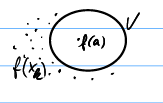
\includegraphics[width=3 cm,height=2cm]{bsp kap 13.4}
	\end{figure}\\ 
	\hfill$\square$\\
	\textbf{13.5. \underline{Beh.:}} \greenul{f stetig}\\
	$\Leftrightarrow$ [\greenul{$O \in \mathcal{O}(\sigma)\Rightarrow f^{-1}(O)\in \mathcal{O}(S)$}] "\redul{Urbilder offener Mengen sind offen.}"\\
	$\Leftrightarrow$[\greenul{$A\in \mathcal{A}(\sigma)\Rightarrow f^{-1}(A)\in \mathcal{A}(S)$}] "\redul{Urbild abg. Mengen sind abg.}"\\
	\underline{Bew.: 1. Zeile "$\Leftarrow$"}: $\OE \overset{\circ}{V}=V \in \mathcal{U}_{f(a)},$ dann $\exists U \in \mathcal{U}_a:f(U)\subseteq V,$ wobei $U\subseteq f^{-1}(v)\in \mathcal{U}_a,$ U offen, also $f^{-1}(V)$ offen.\\
	"$\Rightarrow$": Sei O $\in \mathcal{O}(\sigma)$, wähle $b\in O$ mit $b\in O$ mit $b \in f (R), b= f(a), a\in R.$ \\
	Da f  stetig und $O\in \mathcal{U}_{f(a)} \Rightarrow \exists U_a$ offen, $f(U_a)\subseteq O$ für alle b und alle a mit f(a)=b.\\
	$\Rightarrow f^{-1}(O)\supseteq \bigcup_{a\in f^{-1}(O)} U_a \Rightarrow f^{-1}(O)=\bigcup_{a\in f^{-1}(O)}U_a$ offen.\\
	\underline{2. Zeile:} Für A=$\mathcal{C}O$ ist $f^{-1}(A)=f^{-1}(\mathcal{C}O)=\mathcal{C}f1{-1}(O)$ abg.\\
	\\
	\textbf{13.6. \underline{Stetigkeit bei Kompositionen:}}\\
	\underline{Vor.:} $(R,S) \xrightarrow{f} (S,\sigma) \xrightarrow{g}(T,\uptau),$ \greenul{f,g stetig.}\\
	\underline{Beh.:} \greenul{$g\circ f$ stetig.}\\
	\underline{Bew.:} Für $O \in \mathcal{O}(\uptau)$ ist $(g\circ f)^{-1}(O)=f^{-1}(g^{-1}(O))$ offen, mit \blueul{13.5.} folgt die Beh.\\
	\strut\hfill$\square$\\
	\textbf{13.7. \underline{Trivialität:}} (1)f \greenul{stetig}, $D\subseteq R \Rightarrow$ \greenul{$f_{rD}$ stetig.}\\
	(2) f \greenul{Konstant} $\Rightarrow$ f \greenul{stetig.}\\
	\\
	Erinnerungen an Kapitel \blueul{an 3:}\\
	\textbf{13.8. \underline{Beh.:}} $\mathbb{R}^n \supseteq D \xrightarrow{f} \mathbb{R}^m$ stetig $\Leftrightarrow$ $\forall j: f_j:=pr_j\circ f$ stetig, wo $D\xrightarrow{f}\mathbb{R}^m\xrightarrow{pr_j}\mathbb{R}.$ Vgl. \blueul{an 3.5.}\\
	\\
	\textbf{13.9. \underline{Beh.:}} $(R,||\cdot||)$ normierter $\mathbb{R}-VR \Rightarrow ||\cdot||: R\rightarrow [0,\infty[$ stetig. (Vgl. \blueul{Blatt 2, A3.1}).\\
	\\
	\textbf{13.10. \underline{Beh.:}} $A\in Hom(\mathbb{R}^n, \mathbb{R}^m)$ ist stetig (bzgl. einer von einer Norm induzierten Metrik).\\
	\textopencorner Vgl. mit \blueul{an 3.18}: "K" im dortigen Beweis nennen wir jetzt $||(A)||_\infty$. \textcorner\\
	\underline{Bew.:} Sei $A=(\alpha_{ij}) \in \mathbb{R}^{m\times n}$. Dann gilt $||Ax||_\infty =\underbrace{(\max_{i\in\{1,...,m\}}\sum_{j=1}^{n} |\alpha_{ij}|)}_{=:||A||_\infty}\cdot ||x||_\infty.$\\
	\\
	Mit der Abschätzung \oraul{$||Ax||_\infty \leq ||a||_\infty\cdot||x||_\infty$} mit der Def. für $||A||_\infty$ wie oben gilt also: $\forall x,y \in \mathbb{R}^n: ||Ax-Ay||_\infty=||A(x-y)||_\infty\leq ||A||_\infty \cdot ||x-y||_\infty,$ woraus sofort die Stetigkeit von $A\in Hom(\mathbb{R}^n,\mathbb{R}^m)$ folgt.\\
	\strut\hfill$\square$\\
	\textbf{13.11. \underline{Bem.:}} Die hier gemachte Def. für $||A||_\infty$ als \yelul{$||A||_\infty$} := $\max_{i\in\{1,...,m\}}\sum_{j=1}^{n} |\alpha_{ij}|$ ist sinnvoller als die sonst naheligende Setzung als $\max_{i,j}|\alpha_{ij}|$, da wir früher in \blueul{4.26} und \blueul{5.12} gemacht haben. Die Stetigkeit hängt unmittelbar mit $||A||_\infty$ zusammen. Man nennt $||A||_\infty$ auch die \redul{Operatornorm} von A (bzgl. $||\cdot||_\infty$).\\
	\\
	\textbf{13.12. \underline{Def.:}} \yelul{$||A||_{op}$} := $\inf \{c\geq 0; ||Ax||_V \leq c||x||_W\textbf{für alle} x\in V\}$ heißt \redul{Operatornorm von A}$\in Hom(V,W)$, wo $(V,||\cdot||_V), (W,||\cdot||_W)$ normierte $\mathbb{R}-VR$ seien.\\
	\underline{Bem.:}$\bullet$ Für $A\in Hom(\mathbb{R}^n,\mathbb{R}^m)$ ist \greenul{$||A||_{op}=||A||_\infty$} (für die Norm $||\cdot||_\infty$ auf $\mathbb{R}^n$ und $\mathbb{R}^m$), und $||A||_{op}=\sup \{||Ax||_\infty; x\in \mathbb{R}^n,||x||_\infty=1\}=\sup\{\frac{||AX||_\infty}{||x||_\infty}; x\in\mathbb{R}^n\backslash\{0\}\}.$\\
	$\bullet(Hom(\mathbb{R}^n,\mathbb{R}^m),||\cdot||_{op})$ ist ein normierter VR. \\
	\textopencorner Ohne Beweis, bwz. \redcircle{Ü}, bzw. [\blueul{Funktionalanalysis}]\textcorner\\
	\\
	\textbf{13.13. \underline{Satz:}} \underline{Vor.:} \greenul{D$\subseteq$ R}, \greenul{D Kompakt}, f: \greenul{$R\rightarrow S$ stetig}.\\
	\underline{Beh.:} \greenul{f(D) Kompakt}. "\redul{Bilder Kompakter Mengen sind Kompakt}\\
	\underline{Bew.:} Mit $f(D) = f_{rD}(D)$ betrachte \OE D=R. Sei offene Überdeckung von f(R) vorgegeben, etwa $f(R)=\bigcup_{O\in\mathcal{O}_1}O$. \underline{Z.z.:} endlich viele $O_j\in\mathcal{O}_1$ reichen aus.\\
	Es ist $\bigcup_{O\in\mathcal{O}_1}\underbrace{f^{-1}(O)}_{\text{offen, da f stetig}}$\oraul{$\supseteq R$}, R Kompakt nach Vor.\\
	es folgt: $\exists t$ viele i, etwa $i\in \{1,...,t\}:R\subseteq \bigcup_{i=1}^tf^{-1}(O_i),O_i\in\mathcal{O}_1\\
	\Rightarrow$ \oraul{$f(R)$}$\subseteq \bigcup_{i=1}^tf(f^{-1}(O_i))=\bigcup_{i=1}^tO_i.$\\
	\\
	\textbf{13.14. \underline{Spezialfall:}} $S=\mathbb{R}^n$, dann ist \greenul{f(D) beschränkt und abgeschlossen}.\\
	Falls \underline{n=1}: $\exists d_1,d_2\in D:$ \greenul{$f(d_1)\leq f(d)\leq f(d_2)$} für alle $d \in D$, wobei also $f(d_1)=\min_{d\in D} f(d), f(d_2)=\max_{d\in D}f(d).$\\
	Wir erhalten wieder den bekannten \blueul{Satz von Min./Max An.30} zurück.\\
	Dies rechtfertigt nachträglich die \greenul{Existenz von Extrema von Funktionen} mit NBen, da die Nebenbedingungen in der Form \greenul{N}=$\bigcup_{i=2}^l f^{-1}(O)$ \underline{meistens} \greenul{Kompakt} sind.\\
	Benutzt haben wir dies u.a. in \blueul{9.8.,9.9.,9.10.,9.20.}\\
	\\
	Ein weiterer wichtiger Satz ist die gleichmäßige Stetigkeit von stetigen Fktn. auf Kompakta, vgl. \blueul{An10.8.}\\
	\\
	\textbf{13.15. Satz:} \underline{Vor.:} \greenul{R Kompakt, $f:R\rightarrow S$ stetig.}\\
	\underline{Beh.:} f \greenul{gleichmäßig stetig,} d.h. \greenul{$\forall \epsilon \textgreater0 \exists \delta \textgreater0 \forall x,y \in R: s(x,y)\textless \delta\Rightarrow \sigma(f(x),f(y))\textless \epsilon$}.\\
	\underline{Bew.:} Sei $\epsilon\textgreater0$. Aus der Stetigkeit von f folgt\\
	$\forall x \in R \exists \delta_x\textgreater0: f(B_x^{2\delta_x})\subseteq B_{f(x)}^{\epsilon/2}$.\\
	Es ist \oraul{$R\subseteq \bigcup_{x\in R}B_x^{\delta_x}$}. Da \oraul{R Kompakt} ist, folgt $R \subseteq$ \oraul{$\bigcup_{i=1}^nB_{x_i}^{\delta_{xi}}$}.\\
	Setze \oraul{$\delta:=\min_{i\in\{1,...,n\}}\delta_{x_i}$}$\textgreater 0.$\\
	Ferner wähle x,y so, dass \oraul{$S(x,y)\textless \delta$}.\\
	dann $\exists x_i\in\{x_1,...,x_n\}: x\in B_{x_i}^{\delta_{x_i}}$.\\
	Es ist also $S(x,x_i)\textless\delta_{x_i}$, und ferner ist \oraul{$S(x,y)\textless\delta\leq \delta_{x_i}$},\\
	sodass $S(x_i,y) \leq$ \oraul{$S(x_i,x$}+ \oraul{$S(x,y)\textless 2\delta_{x_i}$} folgt.\\
	Nach Konstruktion von $\delta_{x_i}$, ist \oraul{$\sigma(f(x_i), f(y))\textless \frac{\epsilon}{2}$},\\
	ebenso ist \oraul{$\sigma(f(x),f(x_i))\textless\frac{\epsilon}{2}$}, so dass folgt:\\
	\oraul{$\sigma(f(x),f(y))$}$\leq \sigma(f(x),f(x_i))+\sigma(f(x_i),f(y))$\oraul{$\textless\epsilon$}.\\
	Dies zeigt die \oraul{gleichmäßige Stetigkeit}.\\
	\\
	Die allgemeinste Def. für einen Funktionsgrenzwert für eine Fkt. f zwischen metrischen Räumen lautet wie folgt:\\
	\\
	\textbf{13.16. \underline{Def.:}} Sei \redul{$M\subseteq R, a \in \dot{M}, b\in S, f:R\rightarrow S$}.\\
	Wir sagen, \redul{$f(x)\rightarrow$} Konvergiert/strebt gegen b/ $\lim\limits_{x\rightarrow a}f(x)=b$ \redul{in M}, wenn: \yelul{$f(x)\xrightarrow{x\rightarrow a}b$ für $x\in M$}: $\Leftrightarrow \forall \epsilon \textgreater 0 \exists \delta \textgreater 0 \forall x \in M: S(x,a)\textless \delta \Rightarrow \delta (f(x),b)\textless \epsilon.$\\
	\\
	Wie schon in Analysis I, \blueul{An10.4}, gibt es den folgenden Zusammenhang zwischen Funktionsgrenzwerten und stetigen Fortsetzungen:\\
	\\
	\textbf{13.17. \underline{Vor.:}} $\overline{f}:=\begin{cases}
		f \text{auf} M\backslash\{a\}\\
		b \text{für} x=a
	\end{cases}$\\
	\underline{Beh.:} $f(x)\xrightarrow{x\rightarrow a}b$ für $x\in M \Leftrightarrow \tilde{f}$ stetig in a. \textopencorner $\tilde{f}$ heißt \redul{st. Forts. von f in a}\textcorner\\
	\\
	\textbf{13.18. \underline{Bem.:}} $f(x)\xrightarrow{x\rightarrow a}b$ für $x \in M \Leftrightarrow \forall (x_n) \subseteq M, x_n \rightarrow a: f(x_n)\rightarrow b.$
	
	
	
\end{document}